
% \usepackage{environ}
% \DeclareMathAlphabet{\mathcal}{OMS}{cmsy}{m}{n}
% \SetMathAlphabet{\mathcal}{bold}{OMS}{cmsy}{b}{n} %for big-O

%\beamerdefaultoverlayspecification{<+->}

% \makeatletter
% \newsavebox{\measure@tikzpicture}
% \NewEnviron{scaletikzpicturetowidth}[1]{%
%   \def\tikz@width{#1}%
%   \def\tikzscale{1}\begin{lrbox}{\measure@tikzpicture}%
%   \BODY
%   \end{lrbox}%
%   \pgfmathparse{#1/\wd\measure@tikzpicture}%
%   \edef\tikzscale{\pgfmathresult}%
%   \BODY
% }
% \makeatother

\tikzset{c/.style={every coordinate/.try,draw=#1!50!white}} %set for coord shift hack
%%%%%%%%%%%%%%%
\tikzset{%
    %%%%keep
    node_style_blank/.style={circle,font=\sffamily\scriptsize\bfseries},
    %%%%%%uncomment to hide labels
    node_styleG/.style={circle, draw=black,fill=black,font=\sffamily\scriptsize\bfseries},
    node_styleB/.style={circle, draw=black,fill=black,font=\sffamily\scriptsize\bfseries},
    node_styleR/.style={circle, draw=black,fill=black,font=\sffamily\scriptsize\bfseries}
    %%%%uncomment to show labels
    % node_styleG/.style={append after command={\pgfextra{\node [right] at (\tikzlastnode.mid east) {\tikzlastnode};}
    %  }, circle, draw=black,fill=black,font=\sffamily\scriptsize\bfseries},
    % node_styleB/.style={append after command={\pgfextra{\node [right] at (\tikzlastnode.mid east) {\tikzlastnode};}
    %  },circle, draw=black,fill=black,font=\sffamily\scriptsize\bfseries},
    % node_styleR/.style={append after command={\pgfextra{\node [right] at (\tikzlastnode.mid east) {\tikzlastnode};}
    %  },circle, draw=black,fill=black,font=\sffamily\scriptsize\bfseries},
}

%%%%%
\begin{frame}{The Art Gallery Problem}
    \begin{figure}
        \centering
        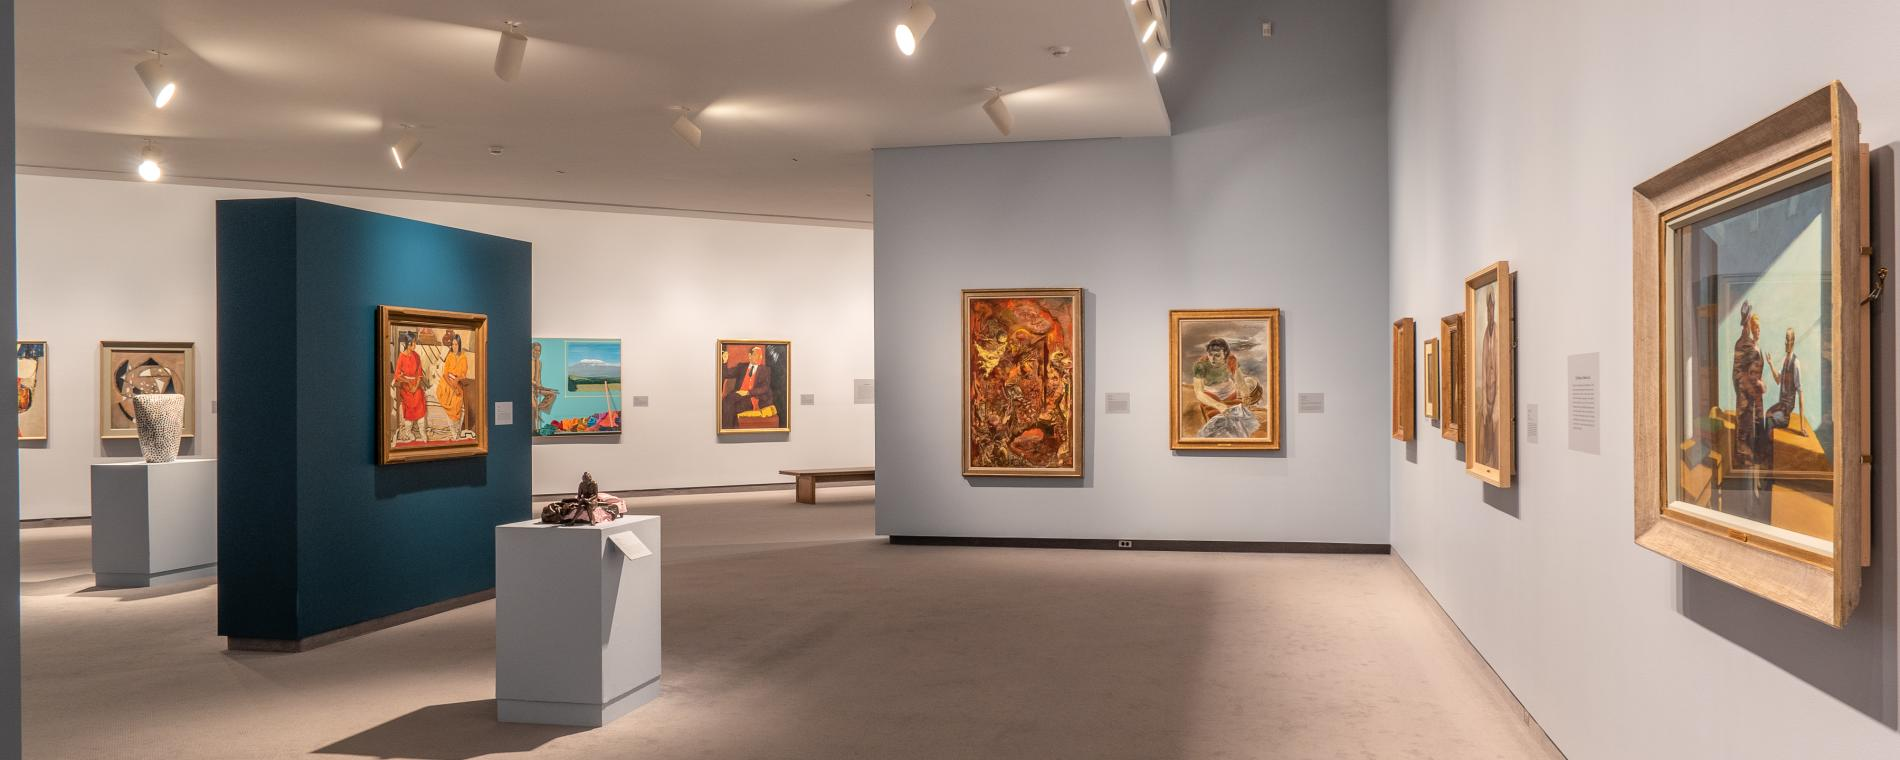
\includegraphics[width=\textwidth]{./images_women_in_IT/Visit_Wichita_Kansas_Wichita_Art_Museum_ab2f81d5-0500-4ccd-af3a-20835143dc89.jpg}
    \end{figure}
\end{frame}

%%%%%
\begin{frame}{How many guards to guard the gallery? Easy case} \label{slide-backstory}
    \def\scalePoly{2}
    \begin{center}
        \only<1>{%
            \begin{tikzpicture}[scale=\scalePoly]
                % create the node
                \node[ultra thick,draw,minimum size=6cm,regular polygon,regular polygon sides=10] (a) {};
                % draw a black dot in each vertex
                \foreach \x in {1,2,...,10}
                  \fill (a.corner \x) circle[radius=2pt];
                % \foreach \x in {2,...,10}
                %   \draw[dashed,<-,red,thick] (a.corner \x) to (a.corner 1);
                % \draw[fill=red] (a.corner 1) circle(.05cm) ;
            \end{tikzpicture}
        }
        \only<2>{%
            \begin{tikzpicture}[scale=\scalePoly]
                % create the node
                \node[ultra thick,draw,minimum size=6cm,regular polygon,regular polygon sides=10] (a) {};
                % draw a black dot in each vertex
                \foreach \x in {1,2,...,10}
                  \fill (a.corner \x) circle[radius=2pt];  
                % \foreach \x in {2,...,10}
                %   \draw[dashed,<-,red,thick] (a.corner \x) to (a.corner 1);
                \draw[fill=red] (a.corner 1) circle(.05cm) ;
            \end{tikzpicture}
        }
        \only<3>{%
            \begin{tikzpicture}[scale=\scalePoly]
                % create the node
                \node[ultra thick,draw,minimum size=6cm,regular polygon,regular polygon sides=10] (a) {};
                % draw a black dot in each vertex
                \foreach \x in {1,2,...,10}
                  \fill (a.corner \x) circle[radius=2pt];
                \foreach \x in {2,...,10}
                  \draw[dashed,<-,red,thick] (a.corner \x) to (a.corner 1);
                \draw[fill=red] (a.corner 1) circle(.05cm) ;
            \end{tikzpicture}
        }
    \end{center}
% No time for that\dots
\end{frame}

%%%%%%%%%%%%%%
\begin{frame}{Most guards needed to guard the gallery? fun case} \label{slide-problem}
        \def\scaleGraph{.65}
        \def\nodeA{\node[node_styleG,] (A) at (-3,4.5) {}}
        % \def\nodeAgreen{\node[node_style, fill = green!50] (A) at (-4,0) {A}}
        \def\nodeB{\node[node_styleB] (B) at (-1.5,2.5) {}}
        \def\nodeC{\node[node_styleG] (C) at (-4.5,1) {}}
        \def\nodeD{\node[node_styleR] (D) at (-2,-4.5) {}}
        % \def\nodeDred{\node[node_style, fill = red!50] (D) at (4,-1) {D}}
        \def\nodeE{\node[node_styleG] (E) at (4.5,-3) {}}
        % \def\nodeEred{\node[node_style, fill =red!50] (E) at (3,3) {E}}
        \def\nodeF{\node[node_styleB] (F) at (4,2) {}}
        \def\nodeG{\node[node_styleR] (G) at (1.5,1) {}}
        \def\nodeH{\node[node_styleB] (H) at (-1.5,-3) {}}
        \def\nodeI{\node[node_styleR] (I) at (-1.5,1) {}}
        \def\nodeJ{\node[node_styleG] (J) at (0.425,0.5) {}}
        \def\nodeK{\node[node_styleR] (K) at (0.5,3.5) {}}
        %%%%
    \begin{center}
    \only<1>{%
        \centering
        \vfill
        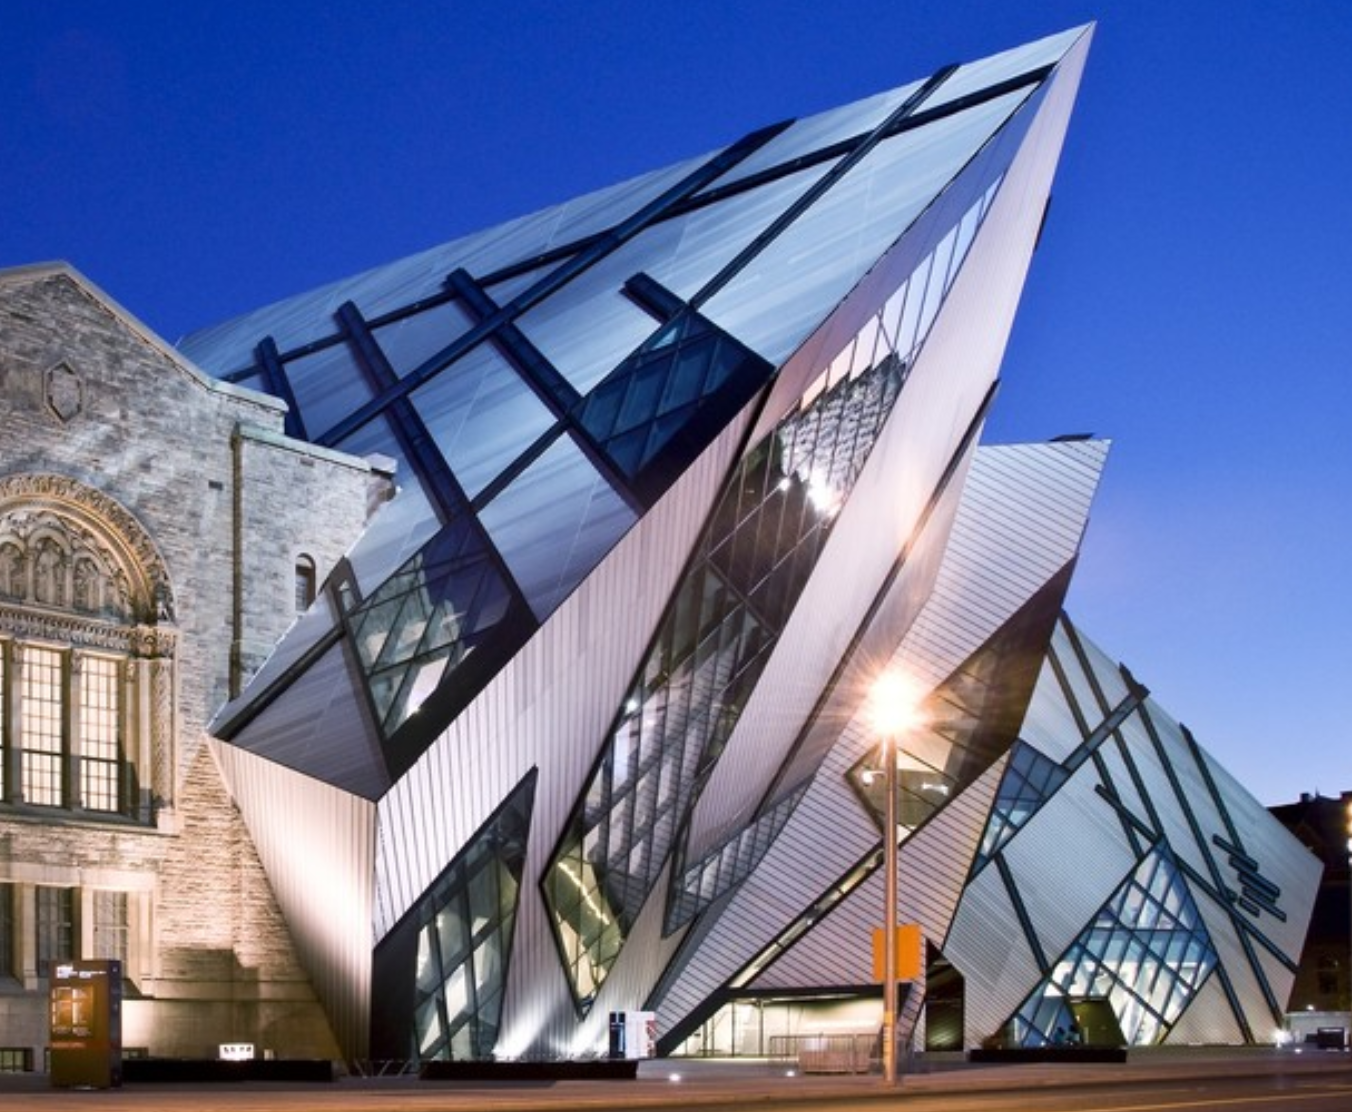
\includegraphics[width=.65\textwidth]{./images_women_in_IT/toronto_art_gallery.png}
    }
    \only<2>{%
        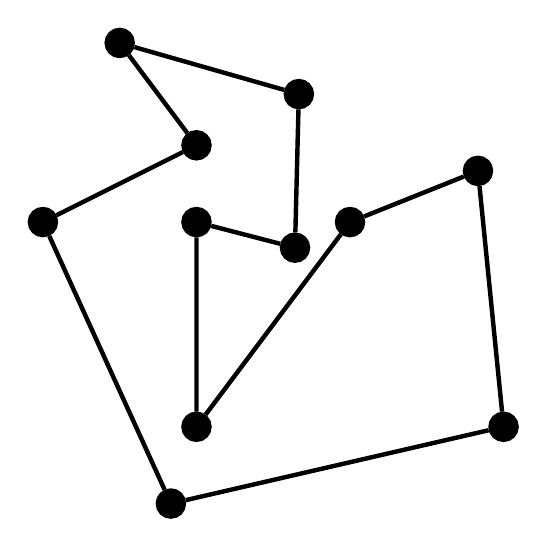
\begin{tikzpicture}[scale=\scaleGraph,shorten >=0pt, auto, node distance=3cm, ultra thick, edge_style/.style={draw=black, ultra thick},label_style/.style={fill=white,text opacity =.5, anchor=center, pos=0.5}] 
            \nodeA;
            \nodeB;
            \nodeC;
            \nodeD;
            \nodeE;
            \nodeF;
            \nodeG;
            \nodeH;
            \nodeI;
            \nodeJ;
            \nodeK;
            \draw[ultra thick,black] (A) -- (B) -- (C) -- (D) -- (E) -- (F) -- (G) -- (H) -- (I) -- (J) -- (K) -- (A);
        % \draw[ultra thick, draw black] (A)-(B)
        \end{tikzpicture}
    }
    \only<3>{%
    Original proof by V.\ Chvital (1975)
    \begin{figure}
        \centering
        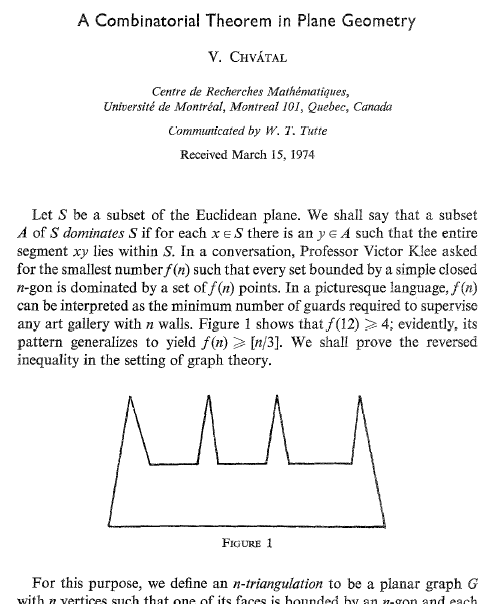
\includegraphics[width=.45\textwidth]{./images_women_in_IT/original_art_gallery_proof-1.png}
    \end{figure}
    }
    \only<4>{%
    Original proof by V.\ Chvital (1975)
    \begin{figure}
        \centering
        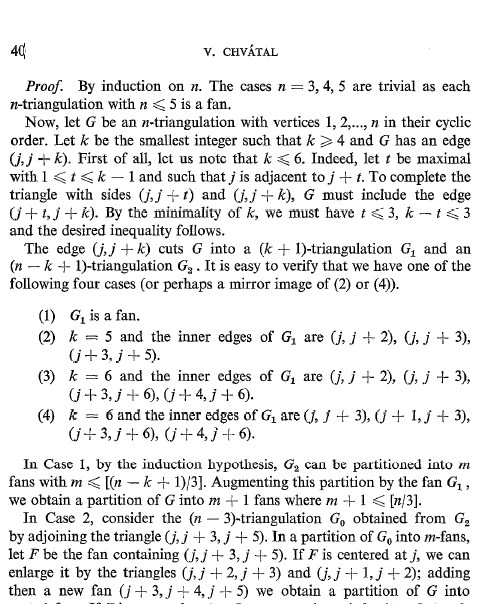
\includegraphics[width=.45\textwidth]{./images_women_in_IT/original_art_gallery_proof-2.png}
    \end{figure}
    }
    \end{center}
\end{frame}

\begin{frame}{}
        \def\scaleGraph{.65}
        \def\nodeA{\node[node_styleG,] (A) at (-3,4.5) {}}
        % \def\nodeAgreen{\node[node_style, fill = green!50] (A) at (-4,0) {A}}
        \def\nodeB{\node[node_styleB] (B) at (-1.5,2.5) {}}
        \def\nodeC{\node[node_styleG] (C) at (-4.5,1) {}}
        \def\nodeD{\node[node_styleR] (D) at (-2,-4.5) {}}
        % \def\nodeDred{\node[node_style, fill = red!50] (D) at (4,-1) {D}}
        \def\nodeE{\node[node_styleG] (E) at (4.5,-3) {}}
        % \def\nodeEred{\node[node_style, fill =red!50] (E) at (3,3) {E}}
        \def\nodeF{\node[node_styleB] (F) at (4,2) {}}
        \def\nodeG{\node[node_styleR] (G) at (1.5,1) {}}
        \def\nodeH{\node[node_styleB] (H) at (-1.5,-3) {}}
        \def\nodeI{\node[node_styleR] (I) at (-1.5,1) {}}
        \def\nodeJ{\node[node_styleG] (J) at (0.425,0.5) {}}
        \def\nodeK{\node[node_styleR] (K) at (0.5,3.5) {}}
        %%%%
        \def\nodeAa{\node[node_style_blank] (Aa) at (-3,4.5) {}}
        \def\nodeBb{\node[node_style_blank] (Bb) at (-1.5,2.5) {}}
        \def\nodeCc{\node[node_style_blank] (Cc) at (-4.5,1) {}}
        \def\nodeDd{\node[node_style_blank] (Dd) at (-2,-4.5) {}}
        \def\nodeEe{\node[node_style_blank] (Ee) at (4.5,-3) {}}
        \def\nodeFf{\node[node_style_blank] (Ff) at (4,2) {}}
        \def\nodeGg{\node[node_style_blank] (Gg) at (1.5,1) {}}
        \def\nodeHh{\node[node_style_blank] (Hh) at (-1.5,-3) {}}
        \def\nodeIi{\node[node_style_blank] (Ii) at (-1.5,1) {}}
        \def\nodeJj{\node[node_style_blank] (Jj) at (0.425,0.5) {}}
        \def\nodeKk{\node[node_style_blank] (Kk) at (0.5,3.5) {}}
        \normalsize
    %%%%%%
    % \only<1>{%
    %     \begin{tikzpicture}[scale=\scaleGraph,shorten >=0pt, auto, node distance=3cm, ultra thick, edge_style/.style={draw=black, ultra thick},label_style/.style={fill=white,text opacity =.5, anchor=center, pos=0.5}] 
    %         \nodeA;
    %         \nodeB;
    %         \nodeC;
    %         \nodeD;
    %         \nodeE;
    %         \nodeF;
    %         \nodeG;
    %         \nodeH;
    %         \nodeI;
    %         \nodeJ;
    %         \nodeK;
    %         \draw[ultra thick,black] (A) -- (B) -- (C) -- (D) -- (E) -- (F) -- (G) -- (H) -- (I) -- (J) -- (K) -- (A);
    %     \end{tikzpicture}
    % }
    %%%%%%
    \begin{columns}[T]
        \begin{column}{.45\textwidth}
            \centering
                \begin{tikzpicture}[scale=\scaleGraph,shorten >=0pt, auto, node distance=3cm, ultra thick, edge_style/.style={draw=black, ultra thick},label_style/.style={fill=white,text opacity =.5, anchor=center, pos=0.5}] 
                    \only<1-3>{%
                        \nodeA; \nodeB; \nodeC; \nodeD; \nodeE; \nodeF; \nodeG; \nodeH; \nodeI; \nodeJ; \nodeK;
                        \draw[ultra thick,black] (A) -- (B) -- (C) -- (D) -- (E) -- (F) 
                        -- (G) -- (H) -- (I) -- (J) -- (K) -- (A);
                    }
                    \only<4>{%
                        \nodeA; \nodeB; \nodeC; \nodeD; \nodeEe; \nodeFf; \nodeGg; \nodeH; \nodeI; \nodeJ; \nodeK;
                        \draw[ultra thick,black] (A) -- (B) -- (C) -- (D) -- (H) -- (I) -- (J) -- (K) -- (A);
                    }
                    \only<5>{%
                        \nodeA; \nodeB; \nodeC; \nodeD; \nodeEe; \nodeFf; \nodeGg; \nodeH; \nodeI; \nodeJ; \nodeK;
                        \draw[ultra thick,black] (A) -- (B) -- (C) -- (D) -- (H) -- (I) -- (J) -- (K) -- (A);
                        \draw[thick,dashed,blue] (K) -- (B);
                        \draw[thick,dashed,blue] (B) -- (J);
                        \draw[thick,dashed,blue] (I) -- (B);
                        \draw[thick,dashed,blue] (I) -- (C);
                        \draw[thick,dashed,blue] (C) -- (H);
                        % \draw[thick,dashed,black] (H) -- (D);
                        % \draw[thick,dashed,black] (H) -- (E);
                        % \draw[thick,dashed,black] (E) -- (G);
                    }
                    \only<6-8>{%
                        \nodeA; \nodeB; \nodeC; \nodeD; \nodeE; \nodeFf; \nodeGg; \nodeH; \nodeI; \nodeJ; \nodeK;
                        \draw<6-7>[ultra thick,black] (A) -- (B) -- (C) -- (D) -- (H) -- (I) -- (J) -- (K) -- (A);
                        \draw[thick,dashed,blue] (K) -- (B);
                        \draw[thick,dashed,blue] (B) -- (J);
                        \draw[thick,dashed,blue] (I) -- (B);
                        \draw[thick,dashed,blue] (I) -- (C);
                        \draw[thick,dashed,blue] (C) -- (H);
                        \draw<7->[thick,black] (H) -- (E);
                        \draw<8->[thick,black] (E) -- (D);
                        \draw<8>[thick,dashed,blue] (H) -- (D);
                        \draw<8>[ultra thick,black] (A) -- (B) -- (C) -- (D) -- (E) -- (H) -- (I) -- (J) -- (K) -- (A);
        
                    }
                    \only<9-10>{%
                        \nodeA; \nodeB; \nodeC; \nodeD; \nodeE; \nodeFf; \nodeGg; \nodeG; \nodeH; \nodeI; \nodeJ; \nodeK;
                        \draw<9>[ultra thick,black] (A) -- (B) -- (C) -- (D) -- (E) -- (H) -- (I) -- (J) -- (K) -- (A);
                        \draw[thick,dashed,blue] (K) -- (B);
                        \draw[thick,dashed,blue] (B) -- (J);
                        \draw[thick,dashed,blue] (I) -- (B);
                        \draw[thick,dashed,blue] (I) -- (C);
                        \draw[thick,dashed,blue] (C) -- (H);
                        \draw[thick,black] (E) -- (D);
                        \draw[thick,dashed,blue] (H) -- (D);
                        \draw<10->[thick,dashed,blue] (H) -- (E);
                        \draw<10>[ultra thick,black] (A) -- (B) -- (C) -- (D) -- (E) -- (G) -- (H) -- (I) -- (J) -- (K) -- (A);
                        % \draw<11>[ultra thick,black] (A) -- (B) -- (C) -- (D) -- (E) -- (F) -- (G) -- (H) -- (I) -- (J) -- (K) -- (A);
                    }
                    \only<11-14>{%
                        \nodeA; \nodeB; \nodeC; \nodeD; \nodeE; \nodeF; \nodeFf; \nodeGg; \nodeG; \nodeF; \nodeH; \nodeI; \nodeJ; \nodeK;
                        \draw<11>[ultra thick,black] (A) -- (B) -- (C) -- (D) -- (E) -- (G) -- (H) -- (I) -- (J) -- (K) -- (A);
                        \draw[thick,dashed,blue] (K) -- (B);
                        \draw[thick,dashed,blue] (B) -- (J);
                        \draw[thick,dashed,blue] (I) -- (B);
                        \draw[thick,dashed,blue] (I) -- (C);
                        \draw[thick,dashed,blue] (C) -- (H);
                        \draw[thick,black] (E) -- (D);
                        \draw[thick,dashed,blue] (H) -- (D);
                        \draw[thick,dashed,blue] (H) -- (E);
                        \draw<12->[ultra thick,black] (A) -- (B) -- (C) -- (D) -- (E) -- (F) -- (G) -- (H) -- (I) -- (J) -- (K) -- (A);
                        \draw<12->[thick,dashed,blue] (G) -- (E);
                        % \draw<12->[thick,dashed,blue] (G) -- (E);
                    }
                    \only<15->{%
                        \nodeA; \nodeB; \nodeCc; \nodeDd; \nodeEe; \nodeFf; \nodeFf; \nodeGg; \nodeHh; \nodeIi; \nodeJj; \nodeK;
                        \draw[ultra thick,black] (A) -- (B) -- (K) -- (A); 
                    } 
                \end{tikzpicture}
        \end{column}
        %%%%%%%
        \begin{column}{.55\textwidth}
            \begin{block}<2->{Claim:}
                Any shape like this can be \textit{triangulated}.
            \end{block} 
            \begin{itemize}
                \item<3->[] IF we can do it for $N$ vertices. 
                \item<8->[] THEN we can do it for $N+1$ vertices. 
                \item[] 
                \item<13->[] So we just need a starting point$\dots$ 
                \item<14->[] $N=3$ 
            \end{itemize}
        \end{column}
    \end{columns}
\end{frame}

\begin{frame}
        \def\scaleGraph{.65}
        \def\nodeA{\node[node_styleG,] (A) at (-3,4.5) {}}
        % \def\nodeAgreen{\node[node_style, fill = green!50] (A) at (-4,0) {A}}
        \def\nodeB{\node[node_styleB] (B) at (-1.5,2.5) {}}
        \def\nodeC{\node[node_styleG] (C) at (-4.5,1) {}}
        \def\nodeD{\node[node_styleR] (D) at (-2,-4.5) {}}
        % \def\nodeDred{\node[node_style, fill = red!50] (D) at (4,-1) {D}}
        \def\nodeE{\node[node_styleG] (E) at (4.5,-3) {}}
        % \def\nodeEred{\node[node_style, fill =red!50] (E) at (3,3) {E}}
        \def\nodeF{\node[node_styleB] (F) at (4,2) {}}
        \def\nodeG{\node[node_styleR] (G) at (1.5,1) {}}
        \def\nodeH{\node[node_styleB] (H) at (-1.5,-3) {}}
        \def\nodeI{\node[node_styleR] (I) at (-1.5,1) {}}
        \def\nodeJ{\node[node_styleG] (J) at (0.425,0.5) {}}
        \def\nodeK{\node[node_styleR] (K) at (0.5,3.5) {}}
        %%%%
        \normalsize
        \begin{columns}[T]
            \begin{column}{.45\textwidth}
                \centering
                \only<1>{%
                    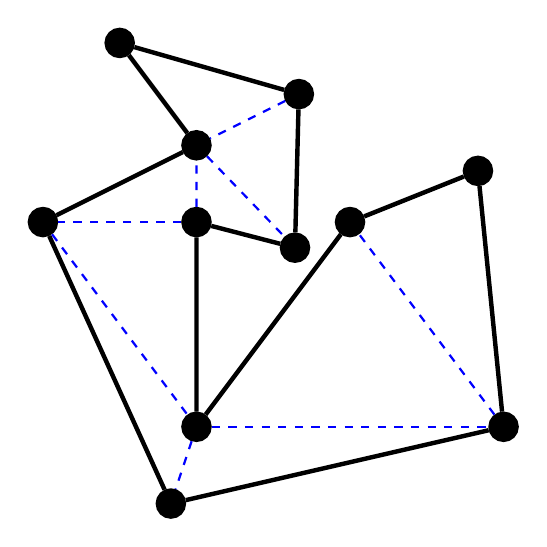
\begin{tikzpicture}[scale=\scaleGraph,shorten >=0pt, auto, node distance=3cm, ultra thick, 
                        edge_style/.style={draw=black, ultra thick},label_style/.style={fill=white,text opacity =.5, anchor=center, pos=0.5}] 
                        \nodeA;
                        \nodeB;
                        \nodeC;
                        \nodeD;
                        \nodeE;
                        \nodeF;
                        \nodeG;
                        \nodeH;
                        \nodeI;
                        \nodeJ;
                        \nodeK;
                        \draw[ultra thick,black] (A) -- (B) -- (C) -- (D) -- (E) -- (F) -- (G) -- (H) -- (I) -- (J) -- (K) -- (A);
                        \draw[thick,dashed,blue] (K) -- (B);
                        \draw[thick,dashed,blue] (B) -- (J);
                        \draw[thick,dashed,blue] (I) -- (B);
                        \draw[thick,dashed,blue] (I) -- (C);
                        \draw[thick,dashed,blue] (C) -- (H);
                        \draw[thick,dashed,blue] (H) -- (D);
                        \draw[thick,dashed,blue] (H) -- (E);
                        \draw[thick,dashed,blue] (E) -- (G);
                        % \draw[ultra thick, draw black] (A)-(B)
                    \end{tikzpicture}
                    }
                \only<2-3>{%
                    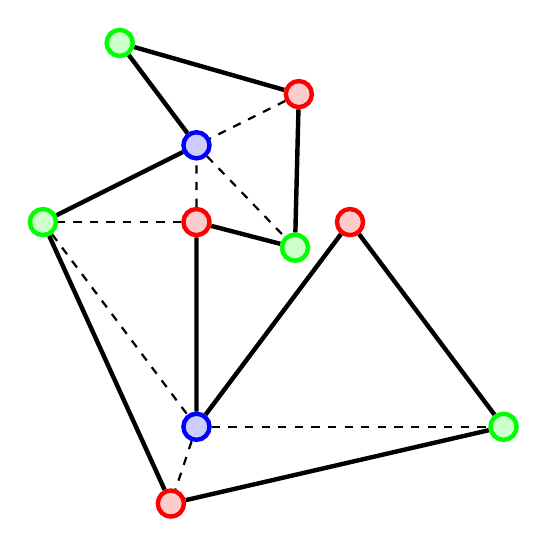
\begin{tikzpicture}[scale=\scaleGraph,shorten >=0pt, auto, node distance=3cm, ultra thick,
                    node_styleG/.style={circle,draw=green,fill=green!20!,font=\sffamily\scriptsize\bfseries},
                    node_styleB/.style={circle,draw=blue,fill=blue!20!,font=\sffamily\scriptsize\bfseries},
                    node_styleR/.style={circle,draw=red,fill=red!20!,font=\sffamily\scriptsize\bfseries},
                    node_style_blank/.style={circle,draw=black,fill=black,font=\sffamily\scriptsize\bfseries},
                    edge_style/.style={draw=black, ultra thick},label_style/.style={fill=white,text opacity =.5, anchor=center, pos=0.5}] 
                        \nodeA;
                        \nodeB;
                        \nodeC;
                        \nodeD;
                        \nodeE;
                        % \nodeF;
                        \nodeG;
                        \nodeH;
                        \nodeI;
                        \nodeJ;
                        \nodeK;
                        
                        \draw[ultra thick,black] (A) -- (B) -- (C) -- (D) -- (E) --  (G) -- (H) -- (I) -- (J) -- (K) -- (A);
                        \draw[thick,dashed,black] (K) -- (B);
                        \draw[thick,dashed,black] (B) -- (J);
                        \draw[thick,dashed,black] (I) -- (B);
                        \draw[thick,dashed,black] (I) -- (C);
                        \draw[thick,dashed,black] (C) -- (H);
                        \draw[thick,dashed,black] (H) -- (D);
                        \draw[thick,dashed,black] (H) -- (E);
                        % \draw[thick,dashed,black] (E) -- (G);
                    % \draw[ultra thick, draw black] (A)-(B)
                    \end{tikzpicture}
                }
                \only<4->{%
                    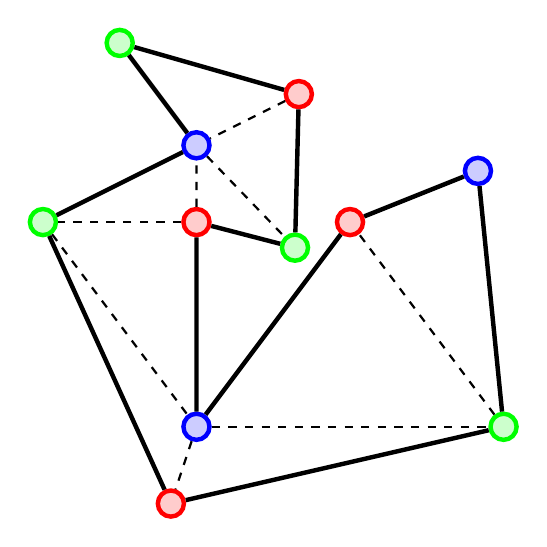
\begin{tikzpicture}[scale=\scaleGraph,shorten >=0pt, auto, node distance=3cm, ultra thick,
                    node_styleG/.style={circle,draw=green,fill=green!20!,font=\sffamily\scriptsize\bfseries},
                    node_styleB/.style={circle,draw=blue,fill=blue!20!,font=\sffamily\scriptsize\bfseries},
                    node_styleR/.style={circle,draw=red,fill=red!20!,font=\sffamily\scriptsize\bfseries},
                    node_style_blank/.style={circle,draw=black,fill=black,font=\sffamily\scriptsize\bfseries},
                    edge_style/.style={draw=black, ultra thick},label_style/.style={fill=white,text opacity =.5, anchor=center, pos=0.5}] 
                        \nodeA;
                        \nodeB;
                        \nodeC;
                        \nodeD;
                        \nodeE;
                        \nodeF;
                        \nodeG;
                        \nodeH;
                        \nodeI;
                        \nodeJ;
                        \nodeK;
                        
                        \draw[ultra thick,black] (A) -- (B) -- (C) -- (D) -- (E) -- (F) -- (G) -- (H) -- (I) -- (J) -- (K) -- (A);
                        \draw[thick,dashed,black] (K) -- (B);
                        \draw[thick,dashed,black] (B) -- (J);
                        \draw[thick,dashed,black] (I) -- (B);
                        \draw[thick,dashed,black] (I) -- (C);
                        \draw[thick,dashed,black] (C) -- (H);
                        \draw[thick,dashed,black] (H) -- (D);
                        \draw[thick,dashed,black] (H) -- (E);
                        \draw[thick,dashed,black] (E) -- (G);
                    % \draw[ultra thick, draw black] (A)-(B)
                    \end{tikzpicture}
                }
        \end{column}
        %%%%%%%
        \begin{column}{.55\textwidth}
            \only<1-4>{%
                \begin{block}<2->{Claim:}
                    Any triangulated shape like can be \textit{tri-colored}.
                \end{block} 
                \begin{itemize}
                    \item<3->[] IF we can do it for $N$ vertices. 
                    \item<4->[] THEN we can do it for $N+1$ vertices. 
                    \item[] 
                    \item<5->[] So we just need a starting point$\dots$ 
                    \item<6->[] $N=3$ 
                \end{itemize}
            }
            \only<5->{%
                \begin{theorem}
                    At most, $\lfloor {\frac{N}{3}} \rfloor$ guards are needed.
                \end{theorem} 
                \begin{itemize}
                    \item<6->[] $\lfloor {\frac{N}{3}} \rfloor$ is just $\frac{N}{3}$ rounded down. 
                    \item<7->[] Since there are $N$ vertices, at least one color will occur $\lfloor {\frac{N}{3}} \rfloor$ times. 
                    \item<8->[] Otherwise the colors would add up to more than $N$. 
                    \item[] 
                    \item<8->[] Post guards at the color! 
                    \item<9->[] In this case \textcolor{blue}{blue}.
                \end{itemize}
                \only<10->{$\frac{11}{3} = 3.666\dots$ so $3$ guards}
            }
        \end{column}
    \end{columns}
\end{frame}

% \begin{frame}
    
%     \uncover<3->{
%         \vspace{-1cm}
        
%         \begin{equation*}
%             \hspace{1cm} \text{At most }\lfloor {\frac{n}{3}} \rfloor \text{ guards.} 
%         \end{equation*}
%         -Fisk's short proof (1978)
%     }
% \end{frame}

%%%%%%%%%%%%%%%
\begin{frame}{} 
\Large
\centering
Proof by Induction
\vspace{10pt}
\large
    \begin{itemize}
        \item<2->[] Assume it's true for $N$.
        \item<3->[] Show it's true for $N+1$ (induction step).
        \item<4->[] Show it's true for any $N$ (base case).
    \end{itemize}
\end{frame}

\begin{frame}{}
    \vspace{10pt}
    \centering
    \begin{figure}
        
\includegraphics[width=.95\textwidth]{./images_women_in_IT/quote-god-has-the-big-book-the-beautiful-proofs-of-mathematical-theorems-are-listed-here-paul-erdos-35-5-0559.jpg}
    \end{figure} 
\end{frame}
